\documentclass[12pt,a4paper]{report}

% =========================================================================
% THU VIEN VA DINH DANG
% =========================================================================
\usepackage{fontspec}
\setmainfont{Times New Roman}
\usepackage[top=2.5cm,bottom=2.5cm,left=3.0cm,right=2.0cm]{geometry}
\usepackage{amsmath,amsfonts,amssymb}
\usepackage{graphicx}
\usepackage{booktabs,tabularx,multirow,array}
\usepackage{float}
\usepackage{xcolor}
\usepackage{tikz}
\usetikzlibrary{calc,positioning,shapes.geometric,arrows.meta}
\usepackage{hyperref}
\usepackage{fancyhdr}
\usepackage{titlesec}
\usepackage{caption}
\usepackage{subcaption}
\usepackage{enumitem}
\usepackage{listings}
\usepackage{tcolorbox}

\graphicspath{{images/generated/}{images/}}

\hypersetup{
    colorlinks=true,
    linkcolor=blue!80!black,
    citecolor=green!60!black,
    urlcolor=blue!70!black,
    pdftitle={Bao Cao Ky Thuat Assignment 06 - RNN Forecasting va Localhost Deployment},
    pdfauthor={khoipv.447}
}

\definecolor{codegreen}{rgb}{0,0.55,0}
\definecolor{codegray}{rgb}{0.45,0.45,0.45}
\definecolor{codepurple}{rgb}{0.58,0,0.82}
\definecolor{backcolour}{rgb}{0.96,0.97,0.98}
\definecolor{reportblue}{RGB}{0,45,145}

\lstdefinestyle{mystyle}{
    backgroundcolor=\color{backcolour},
    commentstyle=\color{codegreen},
    keywordstyle=\color{blue!80!black}\bfseries,
    numberstyle=\tiny\color{codegray},
    stringstyle=\color{codepurple},
    basicstyle=\ttfamily\footnotesize,
    breakatwhitespace=false,
    breaklines=true,
    captionpos=b,
    keepspaces=true,
    numbers=left,
    numbersep=5pt,
    showspaces=false,
    showstringspaces=false,
    showtabs=false,
    tabsize=2,
    frame=single,
    rulecolor=\color{black!20}
}
\lstset{style=mystyle}

\titleformat{\chapter}[display]
  {\normalfont\bfseries\color{reportblue}}
  {\filleft\Large\bfseries\chaptertitlename\ \thechapter}
  {1ex}
  {\titlerule\vspace{1ex}\filright\LARGE}
  [\vspace{1ex}\titlerule]
\titleformat{\section}
  {\normalfont\Large\bfseries\color{blue!70!black}}
  {\thesection}{1em}{}
\titleformat{\subsection}
  {\normalfont\large\bfseries\color{black!85}}
  {\thesubsection}{1em}{}

\pagestyle{fancy}
\fancyhf{}
\fancyhead[R]{\small\itshape Assignment 06: RNN Forecasting và Localhost Deployment}
\fancyfoot[C]{\thepage}
\renewcommand{\headrulewidth}{0.4pt}
\renewcommand{\footrulewidth}{0.4pt}
\setlength{\headheight}{14pt}

\newcommand{\modelpath}[1]{\texttt{#1}}
\newcommand{\best}[1]{\textbf{#1}}
\newcommand{\codeinline}[1]{\texttt{#1}}
\newcommand{\safeimage}[3][\textwidth]{%
  \IfFileExists{images/generated/#2}{\includegraphics[width=#1]{#2}}{%
    \fbox{\parbox[c][6cm][c]{0.92\textwidth}{\centering\bfseries #3}}%
  }%
}

\begin{document}

% =========================================================================
% TRANG BIA
% =========================================================================
\hypersetup{pageanchor=false}
\begin{titlepage}
\thispagestyle{empty}
\begin{tikzpicture}[remember picture,overlay]
    \draw[line width=1.1pt]
      ($(current page.north west)+(1.45cm,-1.35cm)$)
      rectangle
      ($(current page.south east)+(-1.45cm,1.35cm)$);
    \draw[line width=0.35pt]
      ($(current page.north west)+(1.60cm,-1.50cm)$)
      rectangle
      ($(current page.south east)+(-1.60cm,1.50cm)$);
\end{tikzpicture}

\begin{center}
    \textbf{\fontsize{16}{20}\selectfont
    HỌC VIỆN CÔNG NGHỆ BƯU CHÍNH VIỄN THÔNG}\\[0.15cm]
    \textbf{\fontsize{15}{19}\selectfont KHOA CÔNG NGHỆ THÔNG TIN 1}\\[0.25cm]
    \rule{4cm}{0.4pt}

    \vspace{0.75cm}
    
\begin{tikzpicture}
        \node[text=red!80!black,font=\bfseries\fontsize{30}{34}\selectfont,inner sep=1pt] (ptit) {PTIT};
        \node[star,star points=5,star point ratio=2.2,fill=yellow!85!orange,
              draw=yellow!60!black,minimum size=0.72cm,inner sep=0pt]
              at ($(ptit.north)+(0.18cm,-0.06cm)$) {};
        \draw[red!80!black,line width=1.1pt]
            ($(ptit.south west)+(-0.10cm,-0.18cm)$) --
            ($(ptit.south east)+(0.10cm,-0.18cm)$);
        \draw[red!80!black,line width=0.45pt]
            ($(ptit.south west)+(-0.10cm,-0.25cm)$) --
            ($(ptit.south east)+(0.10cm,-0.25cm)$);
    \end{tikzpicture}

    \vspace{0.55cm}
    \textbf{\fontsize{17}{21}\selectfont BÁO CÁO MÔN HỌC}\\[0.25cm]
    \textbf{\fontsize{17}{21}\selectfont PHÁT TRIỂN CÁC HỆ THỐNG THÔNG MINH}\\[0.40cm]
    \textbf{\fontsize{17}{21}\selectfont ASSIGNMENT 06}

    \vspace{1.15cm}
    \begin{tabular}{>{\bfseries}p{3.8cm}p{6.2cm}}
        Họ tên: & Phan Văn Khôi \\
        Mã sinh viên: & B23DCCN447 \\
        Lớp: & D23CTPM01-B \\
        Giảng viên: & PGS. TS. Trần Đình Quế \\
    \end{tabular}

    \vfill
    \textbf{\fontsize{14}{18}\selectfont Hà Nội -- 2026}
\end{center}
\end{titlepage}
\hypersetup{pageanchor=true}

\pagenumbering{roman}
\tableofcontents
\newpage
\listoffigures
\newpage
\listoftables
\newpage
\pagenumbering{arabic}

% =========================================================================
% THONG TIN PROJECT
% =========================================================================
\chapter*{Thông Tin Project}
\addcontentsline{toc}{chapter}{Thông Tin Project}
\noindent\textbf{GitHub project:} \url{https://github.com/KhoiF/PTHTTM}

\vspace{0.4cm}
\noindent Báo cáo tổng hợp kết quả từ hai notebook của Assignment 06:
\begin{itemize}
    \item Amazon Stock Price:\\
    \modelpath{src/Assignment 06/Amazon Stock Price/notebook/}\\
    \modelpath{amazon\_rnn\_forecasting.ipynb};
    \item Avocado Price:\\
    \modelpath{src/Assignment 06/Avocado Price/notebook/}\\
    \modelpath{avocado\_rnn\_forecasting.ipynb}.
\end{itemize}

Hai notebook xây dựng cùng một bài toán dự báo một bước bằng vanilla RNN trên PyTorch và Keras,
đánh giá bằng cùng split thời gian và lưu weights để triển khai. Hai ứng dụng Flask chạy trên localhost
cho phép chọn framework, nạp chuỗi giá gần nhất và thực hiện inference trực tiếp.
Các hình phân tích và đánh giá trong báo cáo được trích từ output đã lưu của notebook.
\newpage

% =========================================================================
% CHUONG 1
% =========================================================================
\chapter{Cơ Sở Lý Thuyết Về RNN}

\section{Chuỗi thời gian và cửa sổ trượt}
Chuỗi thời gian là dãy quan sát có thứ tự
$p_1,p_2,\ldots,p_T$. Khác với dữ liệu độc lập, quan sát tương lai không được dùng để dự báo quá khứ.
Với cửa sổ dài $L$, bài toán được chuyển thành supervised learning:
\begin{equation}
    \mathbf{x}^{(i)}=[p_i,p_{i+1},\ldots,p_{i+L-1}],\qquad
    y^{(i)}=p_{i+L}.
\end{equation}
Amazon dùng $L=60$ phiên giao dịch; Avocado dùng $L=12$ tuần trong từng nhóm region--type.
Các cửa sổ có thể chồng lấn, nhưng target luôn nằm sau toàn bộ input.

\section{Vanilla RNN và hidden state}
Tại thời điểm $t$, RNN kết hợp input mới với bộ nhớ trước đó:
\begin{align}
    \mathbf{a}_t &= \mathbf{x}_tW_{xh}+\mathbf{h}_{t-1}W_{hh}+\mathbf{b}_h,\\
    \mathbf{h}_t &= \tanh(\mathbf{a}_t),\\
    \hat{y} &= W_{hy}\mathbf{h}_L+b_y.
\end{align}
$W_{xh}$ mã hóa quan sát mới; $W_{hh}$ điều khiển thông tin truyền qua thời gian.
Cùng một bộ tham số được dùng tại mọi bước, vì vậy số tham số không tăng theo $L$.
Hai notebook dùng bài toán many-to-one: toàn bộ cửa sổ tạo đúng một dự báo giá kế tiếp.

Với batch, input PyTorch có dạng
$(B,L,d)$, hidden state có dạng $(n_{layer},B,H)$.
Trong thực nghiệm, $d=1$, $H=64$, $n_{layer}=1$ và đầu ra có một phần tử.
Keras có 4,289 tham số; PyTorch có 4,353 tham số do \codeinline{nn.RNN} tách recurrent bias thành hai vector.

\section{Hàm mất mát và BPTT}
Bài toán hồi quy tối ưu Mean Squared Error:
\begin{equation}
    \mathcal{L}=\frac{1}{N}\sum_{i=1}^{N}(y_i-\hat{y}_i)^2.
\end{equation}
Backpropagation Through Time (BPTT) unroll mạng qua $L$ bước, truyền gradient từ output về hidden
state cuối rồi tiếp tục về các hidden state trước đó. Adam sử dụng moment bậc một và bậc hai để cập nhật
tham số; \codeinline{ReduceLROnPlateau} giảm learning rate khi validation loss chững.

\section{Vanishing và exploding gradient}
Gradient qua nhiều bước chứa tích các Jacobian $\partial\mathbf{h}_t/\partial\mathbf{h}_{t-1}$.
Nếu chuẩn tích nhỏ hơn 1, gradient biến mất; nếu lớn hơn 1, gradient bùng nổ.
Đạo hàm $1-\tanh^2(z)$ rất nhỏ khi tanh bão hòa gần $-1$ hoặc $1$.

\begin{figure}[H]
    \centering
    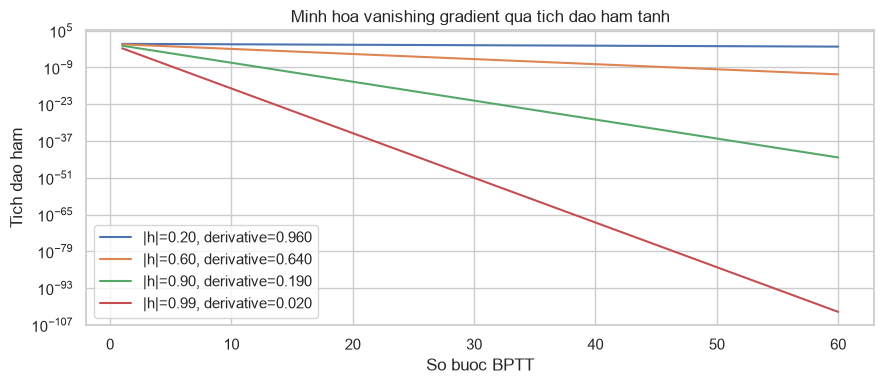
\includegraphics[width=0.88\textwidth]{rnn_vanishing_gradient.png}
    \caption{Minh họa sự suy giảm của tích đạo hàm tanh theo số bước BPTT}
    \label{fig:rnn_vanishing}
\end{figure}

Notebook giảm rủi ro bằng chuẩn hóa input, cửa sổ hữu hạn và gradient clipping với chuẩn tối đa 1.0
trong PyTorch. Dropout 0.2 regularize hidden representation; early stopping chọn weights tốt nhất.

\section{LSTM và GRU}
LSTM bổ sung cell state cùng các cổng input, forget và output để kiểm soát thông tin dài hạn.
GRU gọn hơn với update gate và reset gate. Hai biến thể thường giữ phụ thuộc xa tốt hơn vanilla RNN,
nhưng Assignment 06 dùng vanilla RNN để biểu diễn trực tiếp phương trình hồi quy cơ bản và giữ hai
framework tương đương.

% =========================================================================
% CHUONG 2
% =========================================================================
\chapter{Thiết Kế Thực Nghiệm}

\section{Dataset và nhiệm vụ}
\begin{table}[H]
\centering
\caption{Tổng quan hai dataset của Assignment 06}
\label{tab:dataset_overview}
\resizebox{\textwidth}{!}{%
\begin{tabular}{llllll}
\toprule
\textbf{Dataset} & \textbf{Số dòng} & \textbf{Khoảng thời gian} & \textbf{Target} & \textbf{Lookback} & \textbf{Tần suất} \\
\midrule
Amazon Stock Price & 6,684 & 15/05/1997--05/12/2023 & Close & 60 & Phiên giao dịch \\
Avocado Price & 18,249 & 04/01/2015--25/03/2018 & AveragePrice & 12 & Tuần \\
\bottomrule
\end{tabular}%
}
\end{table}

Amazon là một chuỗi duy nhất. Avocado là panel data gồm 54 region, hai type và 108 chuỗi độc lập.
Mục tiêu của cả hai là dự báo một bước: phiên giao dịch kế tiếp hoặc tuần kế tiếp.

\section{Split theo thời gian và chống data leakage}
Samples được giữ đúng thứ tự, chia xấp xỉ 80\% train, 10\% validation và 10\% test.
Không dùng random split vì thao tác đó có thể đưa quan sát tương lai vào train.

\begin{table}[H]
\centering
\caption{Số mẫu train, validation và test}
\label{tab:split}
\begin{tabular}{lrrr}
\toprule
\textbf{Dataset} & \textbf{Train} & \textbf{Validation} & \textbf{Test} \\
\midrule
Amazon & 5,299 & 662 & 663 \\
Avocado & 13,498 & 1,727 & 1,728 \\
\bottomrule
\end{tabular}
\end{table}

\codeinline{StandardScaler} chỉ fit trên prefix train. Amazon dùng một scaler.
Avocado fit scaler riêng cho từng region--type để giữ thang giá từng thị trường; validation/test chỉ
dùng mean và standard deviation đã học từ train tương ứng.

\section{Kiến trúc và cấu hình huấn luyện}
Cả PyTorch và Keras dùng cùng pipeline:
\begin{equation}
    \text{Sequence}(L,1)
    \rightarrow \text{RNN}(64,\tanh)
    \rightarrow \text{Dropout}(0.2)
    \rightarrow \text{Linear}(1).
\end{equation}

\begin{table}[H]
\centering
\caption{Cấu hình huấn luyện chung}
\label{tab:training_config}
\begin{tabular}{ll}
\toprule
\textbf{Thành phần} & \textbf{Giá trị} \\
\midrule
Optimizer / loss & Adam $10^{-3}$ / MSE \\
Epoch & Tối đa 250, tối thiểu 30 \\
Batch size & 64 \\
Early stopping & Patience 25 theo validation loss \\
Scheduler & Factor 0.5, patience 5 \\
Regularization & Dropout 0.2, gradient clipping 1.0 \\
Random seed & 42 \\
PyTorch device & MPS nếu khả dụng, nếu không dùng CPU \\
\bottomrule
\end{tabular}
\end{table}

\section{Metric đánh giá}
Các metric được tính sau khi inverse-transform về đơn vị giá gốc:
\begin{align}
    \operatorname{MAE}&=\frac{1}{N}\sum_i|y_i-\hat y_i|,\\
    \operatorname{RMSE}&=\sqrt{\frac{1}{N}\sum_i(y_i-\hat y_i)^2},\\
    \operatorname{MAPE}&=\frac{100}{N}\sum_i\left|\frac{y_i-\hat y_i}{y_i}\right|,\\
    R^2&=1-\frac{\sum_i(y_i-\hat y_i)^2}{\sum_i(y_i-\bar y)^2}.
\end{align}
Persistence baseline dùng giá cuối cửa sổ làm giá dự báo và là đối chứng quan trọng cho time series.

% =========================================================================
% CHUONG 3
% =========================================================================
\chapter{Thực Nghiệm Trên Amazon Stock Price}

\section{Khảo sát và chất lượng dữ liệu}
Dataset có các cột Date, Open, High, Low, Close, Adj Close và Volume; không có missing hoặc duplicate.
Giá Close có xu hướng dài hạn mạnh, trong khi phần trăm thay đổi ngày tập trung quanh 0 và có đuôi dày.
Khoảng cách ngày không đều do cuối tuần và ngày nghỉ, nhưng mỗi dòng vẫn đại diện cho một phiên kế tiếp.

\begin{figure}[H]
    \centering
    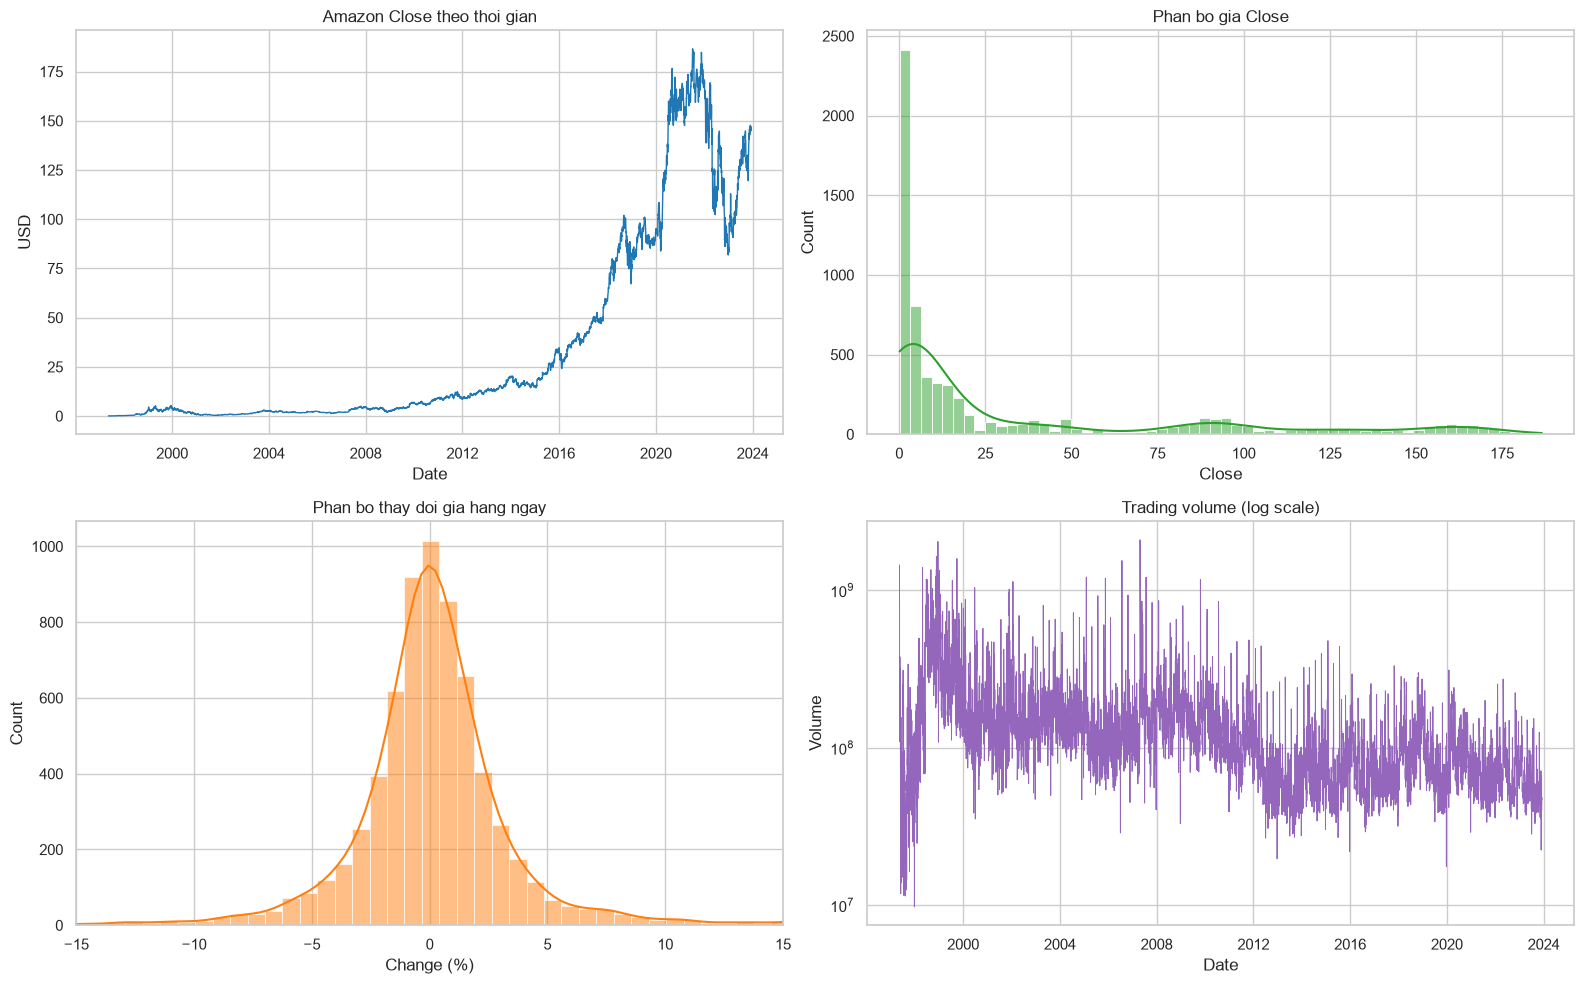
\includegraphics[width=\textwidth]{amazon_eda_overview.png}
    \caption{EDA tổng quan lịch sử giá, phân phối Close, biến động ngày và volume Amazon}
    \label{fig:amazon_eda_overview}
\end{figure}

\begin{figure}[H]
    \centering
    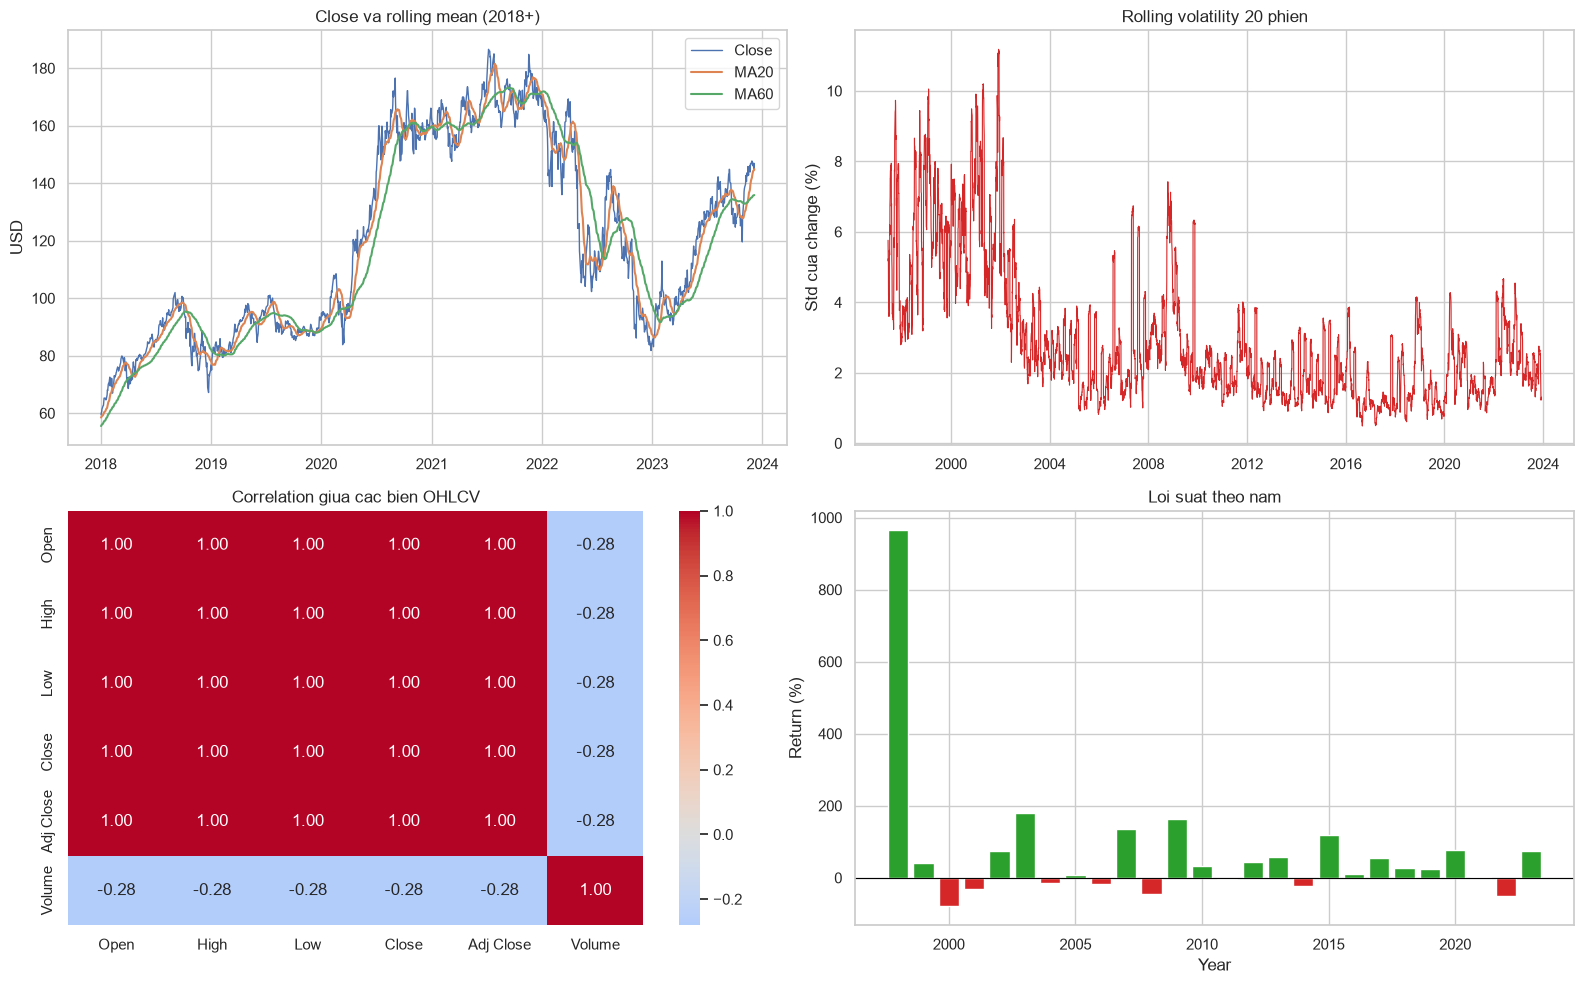
\includegraphics[width=\textwidth]{amazon_eda_diagnostics.png}
    \caption{Rolling statistics, correlation OHLCV và lợi suất năm của Amazon}
    \label{fig:amazon_eda_diagnostics}
\end{figure}

OHLC có tương quan rất cao do cùng mô tả một phiên. Autocorrelation của mức giá Close cũng cao,
nhưng điều này phần lớn phản ánh trend và không có nghĩa chuỗi dừng. Rolling volatility thay đổi mạnh
theo từng regime thị trường.

\section{Tạo sequence và huấn luyện}
Sau lookback 60, dataset tạo 6,624 samples. Scaler train-only có mean 11.5805 và scale 17.4447.
PyTorch chạy 107 epoch, mất 101.50 giây và lưu best validation loss 0.309872.
Keras chạy 75 epoch, mất 18.88 giây. Cả hai best weights được nạp lại độc lập trước khi test.

\section{Kết quả benchmark}
\begin{table}[H]
\centering
\caption{Kết quả test trên Amazon Stock Price}
\label{tab:amazon_results}
\resizebox{\textwidth}{!}{%
\begin{tabular}{lrrrrr}
\toprule
\textbf{Mô hình} & \textbf{MAE} & \textbf{RMSE} & \textbf{MAPE (\%)} & \textbf{$R^2$} & \textbf{Train (s)} \\
\midrule
Persistence baseline & \best{2.2720} & \best{3.1507} & \best{1.7519} & \best{0.9874} & 0.00 \\
PyTorch RNN & 10.4466 & 13.6738 & 6.7825 & 0.7633 & 101.50 \\
Keras RNN & 10.5704 & 14.1749 & 6.8377 & 0.7456 & 18.88 \\
\bottomrule
\end{tabular}%
}
\end{table}

\begin{figure}[H]
    \centering
    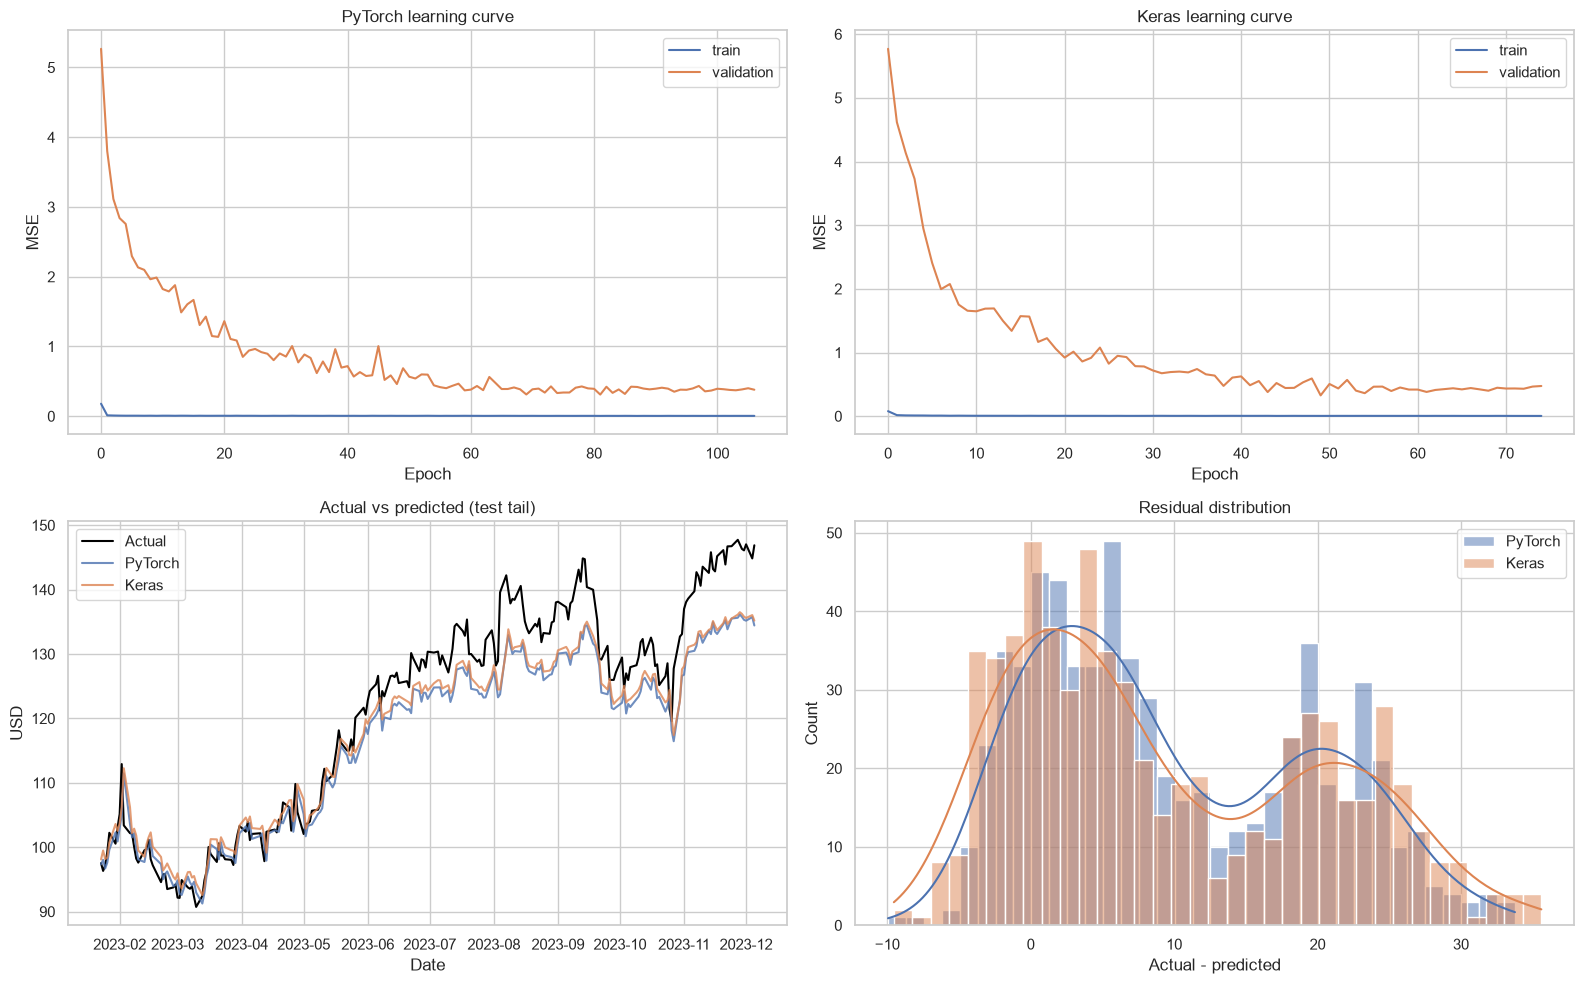
\includegraphics[width=\textwidth]{amazon_model_evaluation.png}
    \caption{Learning curves, actual--predicted và residual trên test Amazon}
    \label{fig:amazon_evaluation}
\end{figure}

Persistence baseline vượt rõ hai RNN. Kết quả này không phải lỗi pipeline: giá cổ phiếu ở dạng mức
có trend mạnh và test nằm ở vùng giá cao hơn nhiều so với phần lớn train. Một RNN tanh nhỏ học trực tiếp
mức giá dễ co dự báo về miền đã quan sát, trong khi baseline tận dụng tính liên tục rất mạnh giữa hai phiên.
Hướng cải thiện phù hợp là dự báo return/difference, rolling normalization hoặc walk-forward retraining.

% =========================================================================
% CHUONG 4
% =========================================================================
\chapter{Thực Nghiệm Trên Avocado Price}

\section{Đặc điểm panel data}
Dataset gồm 18,249 dòng, 169 ngày tuần, 54 region và hai type conventional/organic.
Khóa (Date, region, type) là duy nhất; 107 nhóm có 169 quan sát và một nhóm có 166 quan sát.
Organic thường có giá cao hơn conventional; volume lệch phải và khác nhiều bậc độ lớn giữa các vùng.

\begin{figure}[H]
    \centering
    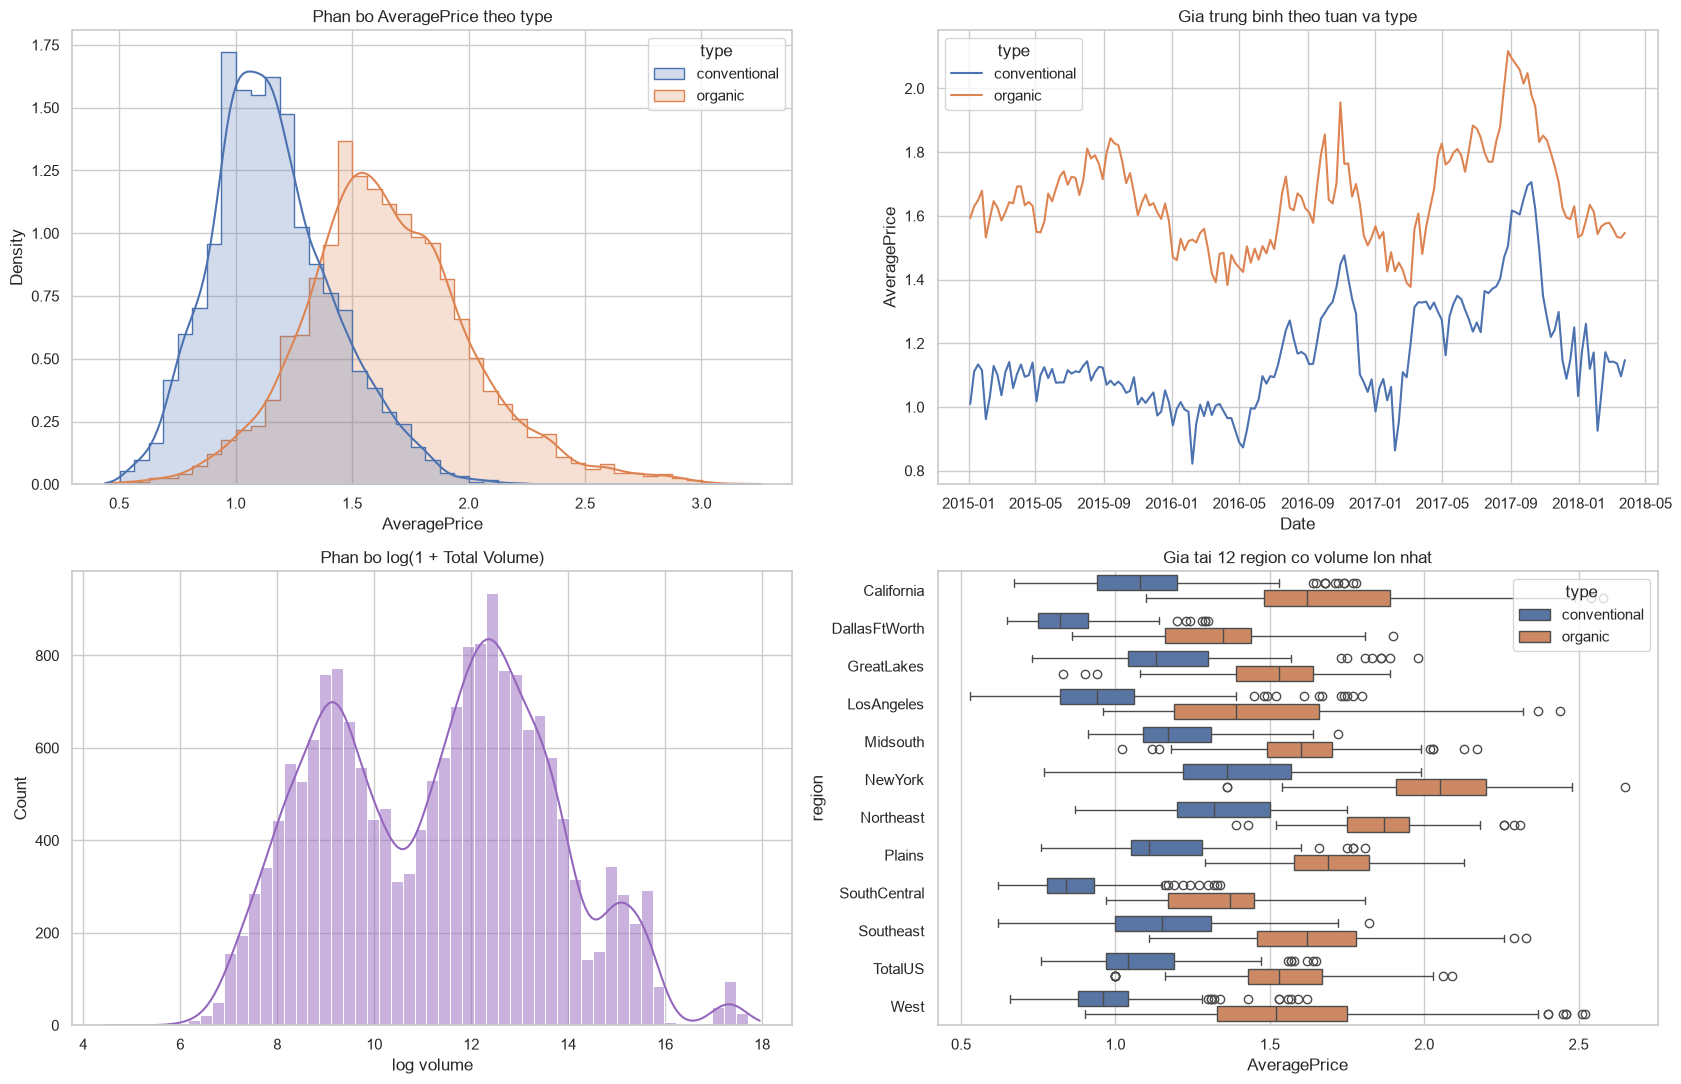
\includegraphics[width=\textwidth]{avocado_eda_overview.png}
    \caption{Phân phối giá, xu hướng tuần, volume và so sánh region của Avocado}
    \label{fig:avocado_eda_overview}
\end{figure}

\begin{figure}[H]
    \centering
    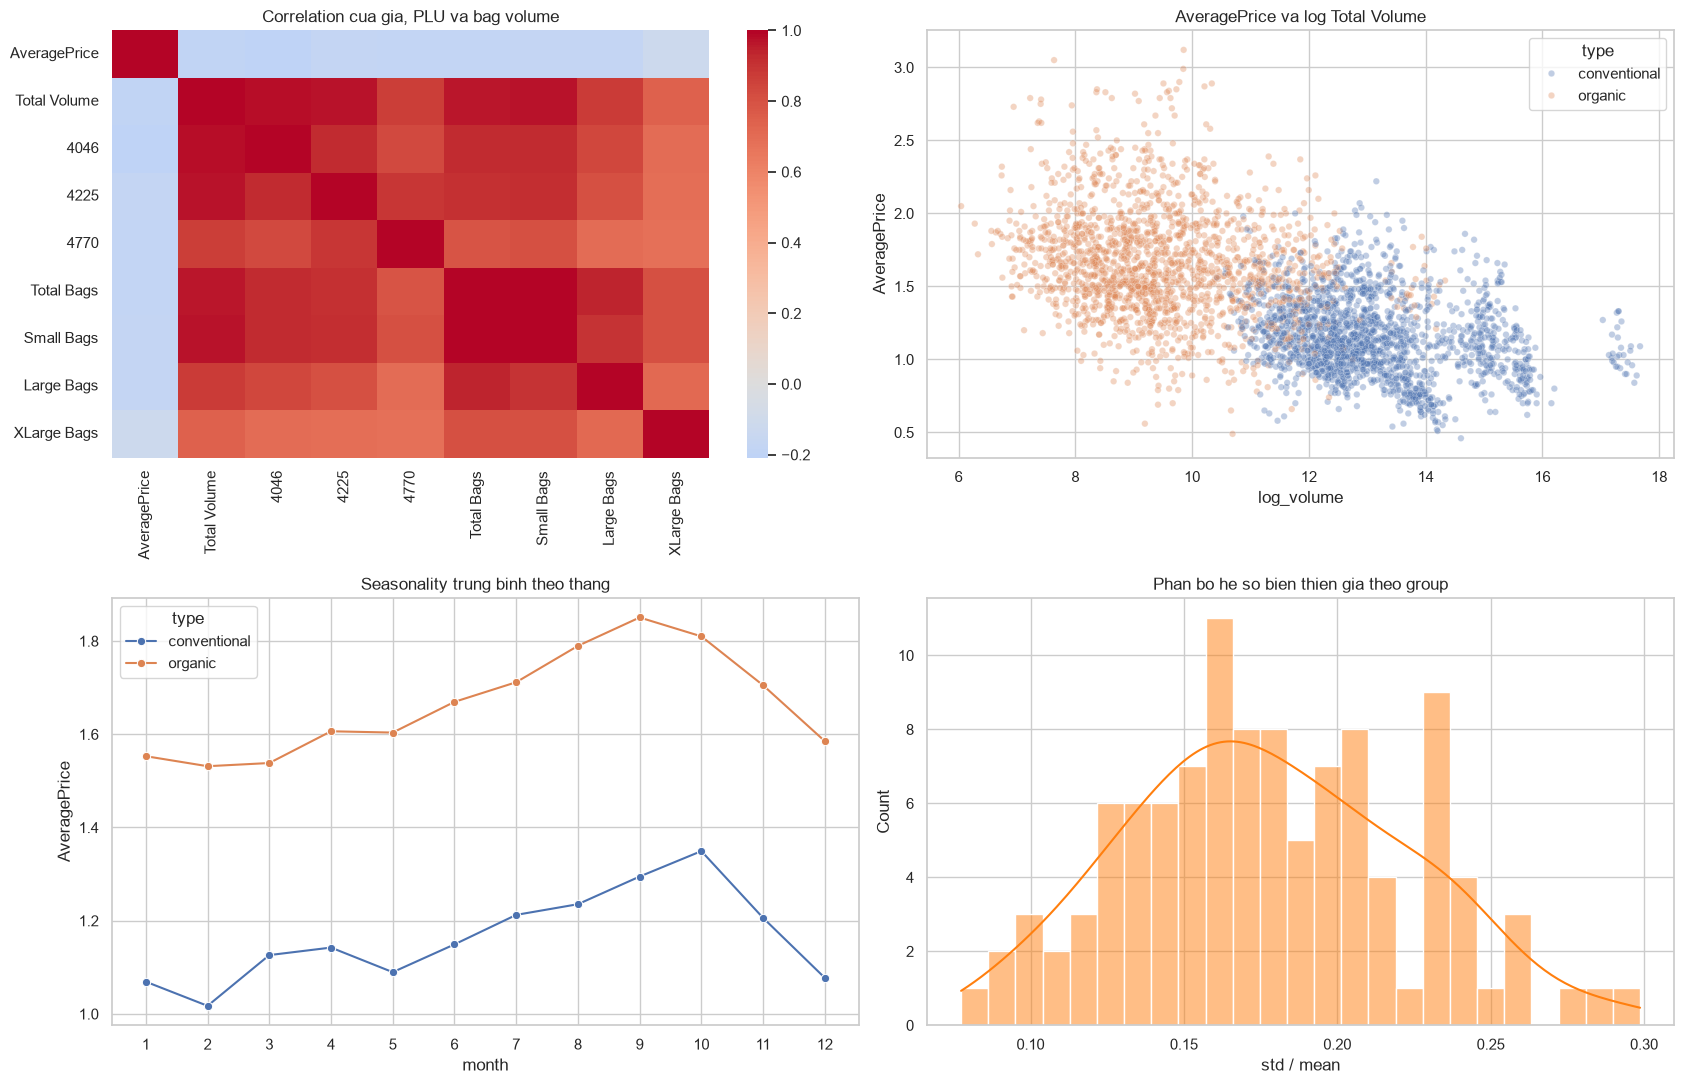
\includegraphics[width=\textwidth]{avocado_eda_diagnostics.png}
    \caption{Correlation, quan hệ giá--volume, seasonality và biến thiên theo nhóm}
    \label{fig:avocado_eda_diagnostics}
\end{figure}

Seasonality cho thấy mức giá thay đổi theo tháng và type. Correlation giữa các cột volume/PLU/bag
phản ánh cấu trúc tổng hợp của dataset; scatter giá--log volume chỉ mang ý nghĩa mô tả, không chứng minh
quan hệ nhân quả.

\section{Tạo sequence theo nhóm và huấn luyện}
Cửa sổ được tạo riêng trong từng region--type nên không đi xuyên ranh giới nhóm. Sau đó samples của
108 nhóm mới được gộp để huấn luyện một RNN chung. PyTorch chạy 32 epoch, mất 22.72 giây và đạt best
validation loss 0.773740. Keras mất 10.88 giây và đạt best validation loss 0.877579.

\section{Kết quả benchmark}
\begin{table}[H]
\centering
\caption{Kết quả test tổng hợp trên 108 chuỗi Avocado}
\label{tab:avocado_results}
\resizebox{\textwidth}{!}{%
\begin{tabular}{lrrrrr}
\toprule
\textbf{Mô hình} & \textbf{MAE} & \textbf{RMSE} & \textbf{MAPE (\%)} & \textbf{$R^2$} & \textbf{Train (s)} \\
\midrule
Keras RNN & \best{0.1099} & \best{0.1534} & \best{8.7926} & \best{0.7490} & 10.88 \\
PyTorch RNN & 0.1122 & 0.1562 & 9.0260 & 0.7398 & 22.72 \\
Persistence baseline & 0.1199 & 0.1742 & 9.5478 & 0.6762 & 0.00 \\
\bottomrule
\end{tabular}%
}
\end{table}

\begin{figure}[H]
    \centering
    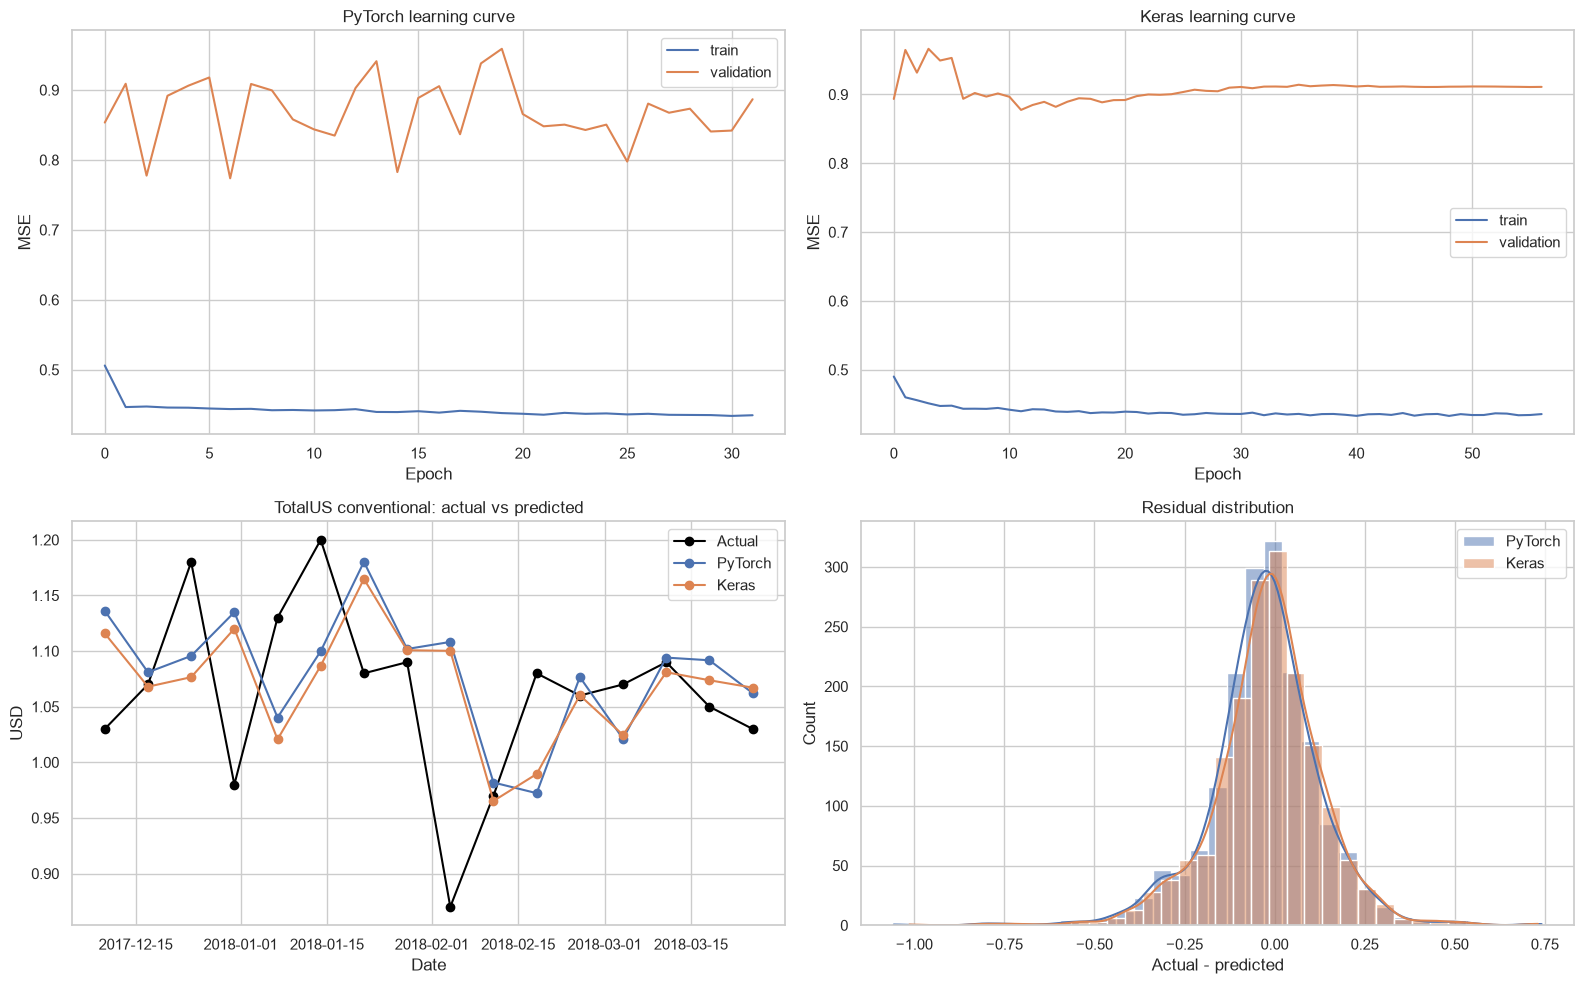
\includegraphics[width=\textwidth]{avocado_model_evaluation.png}
    \caption{Learning curves, dự báo TotalUS--conventional và residual Avocado}
    \label{fig:avocado_evaluation}
\end{figure}

Cả hai RNN vượt persistence baseline trên bốn metric. Keras tốt nhất với RMSE 0.1534 và $R^2=0.7490$.
Chênh lệch giữa hai framework nhỏ; nguyên nhân có thể đến từ cách khởi tạo, bias recurrent và quỹ đạo
optimizer dù kiến trúc/hyperparameter đã được giữ gần tương đương.

% =========================================================================
% CHUONG 5
% =========================================================================
\chapter{Triển Khai Mô Hình Trên Localhost}

\section{Kiến trúc deploy}
Mỗi dataset có một file \codeinline{deploy.py} tự chứa Flask app, HTML/CSS/JavaScript, định nghĩa
kiến trúc RNN và logic nạp weights. Luồng inference gồm:
\begin{equation}
    \text{Web input}
    \rightarrow \text{Validate}
    \rightarrow \text{Scale}
    \rightarrow \text{RNN inference}
    \rightarrow \text{Inverse scale}
    \rightarrow \text{JSON/UI result}.
\end{equation}
Model được cache sau lần nạp đầu. PyTorch ưu tiên MPS khi khả dụng; Keras sử dụng thiết bị TensorFlow
phát hiện. Server chỉ bind \codeinline{127.0.0.1}, phù hợp mục tiêu chạy cục bộ.

\section{Đầu vào và API}
\begin{table}[H]
\centering
\caption{Đầu vào của hai ứng dụng deploy}
\label{tab:deploy_inputs}
\resizebox{\textwidth}{!}{%
\begin{tabular}{lllll}
\toprule
\textbf{Ứng dụng} & \textbf{Framework} & \textbf{Chuỗi giá} & \textbf{Thông tin thêm} & \textbf{Đầu ra} \\
\midrule
Amazon & pytorch / keras & 60 giá Close, cũ $\to$ mới & Không & Close phiên kế tiếp \\
Avocado & pytorch / keras & 12 AveragePrice, cũ $\to$ mới & region, type & AveragePrice tuần kế tiếp \\
\bottomrule
\end{tabular}%
}
\end{table}

Amazon cung cấp \codeinline{POST /api/predict}. Avocado có thêm
\codeinline{GET /api/latest} để đọc 12 tuần mới nhất của nhóm được chọn.
Backend từ chối sai lookback, giá âm, số không hữu hạn, framework hoặc region--type không hợp lệ.

\clearpage
\thispagestyle{fancy}
\section{Giao diện Amazon}
\begin{figure}[H]
    \centering
    \safeimage{amazon_deploy_result.png}{Ảnh giao diện Amazon deploy sau khi dự báo}
    \caption{Giao diện localhost Amazon sau khi dự báo bằng PyTorch}
    \label{fig:amazon_deploy}
\end{figure}

Giao diện tự nạp 60 giá Close cuối từ \codeinline{AMZN.csv}, cho phép đổi framework và hiển thị giá dự
báo cùng device inference. Cổng mặc định là 8001.

\clearpage
\thispagestyle{fancy}
\vspace*{0.5cm}
\section{Giao diện Avocado}
\begin{figure}[H]
    \centering
    \safeimage[0.85\textwidth]{avocado_deploy_result.png}{Ảnh giao diện Avocado deploy sau khi dự báo}
    \caption{Giao diện localhost Avocado cho TotalUS--conventional sau khi dự báo bằng PyTorch}
    \label{fig:avocado_deploy}
\end{figure}

Giao diện cho phép chọn 54 region, hai type và framework. Khi region/type thay đổi, 12 tuần gần nhất
được nạp lại theo nhóm. Cổng mặc định là 8002.

\section{Cách chạy}
Từ thư mục gốc project, kích hoạt môi trường và chạy hai terminal:
\begin{lstlisting}[language=bash,caption={Khởi động hai web deploy trên localhost}]
conda activate ISD
python "src/Assignment 06/Amazon Stock Price/deploy.py" --web
python "src/Assignment 06/Avocado Price/deploy.py" --web
\end{lstlisting}
Sau đó mở một trong hai địa chỉ sau:
\begin{itemize}
    \item Amazon: \url{http://127.0.0.1:8001};
    \item Avocado: \url{http://127.0.0.1:8002}.
\end{itemize}
Dừng server bằng \codeinline{Ctrl+C}. CLI vẫn được giữ để tích hợp tự động hoặc kiểm thử không giao diện.

% =========================================================================
% CHUONG 6
% =========================================================================
\chapter{Tổng Hợp Và Kết Luận}

\section{Tổng hợp kết quả}
\begin{table}[H]
\centering
\caption{Mô hình có RMSE thấp nhất trong từng dataset}
\label{tab:master_summary}
\begin{tabular}{llrrrr}
\toprule
\textbf{Dataset} & \textbf{Mô hình} & \textbf{MAE} & \textbf{RMSE} & \textbf{MAPE (\%)} & \textbf{$R^2$} \\
\midrule
Amazon & Persistence baseline & 2.2720 & 3.1507 & 1.7519 & 0.9874 \\
Avocado & Keras RNN & 0.1099 & 0.1534 & 8.7926 & 0.7490 \\
\bottomrule
\end{tabular}
\end{table}

Amazon cho thấy benchmark time-series phải có persistence baseline: mô hình phức tạp không mặc nhiên
tốt hơn quy tắc giữ giá gần nhất. Avocado cho thấy RNN chung trên các chuỗi được scale theo nhóm có thể
học động lực tuần và cải thiện so với baseline.

\section{Kiểm toán khả năng tái lập}
\begin{table}[H]
\centering
\caption{Checklist tái lập Assignment 06}
\label{tab:reproducibility}
\resizebox{\textwidth}{!}{%
\begin{tabular}{lll}
\toprule
\textbf{Hạng mục} & \textbf{Cách thực hiện} & \textbf{Ý nghĩa} \\
\midrule
Random seed & Seed 42 cho NumPy, Python, PyTorch, Keras & Giảm dao động khởi tạo \\
Split & Theo target time 80/10/10, không shuffle giữa tập & Không nhìn tương lai \\
Scaling & Fit chỉ trên train; Avocado theo nhóm & Chống data leakage \\
Thiết bị & MPS ưu tiên, CPU fallback & Tận dụng Apple Silicon \\
Checkpoint & Lưu best validation loss & Deploy weights tốt nhất \\
Reload test & Dự đoán sau reload khớp notebook & Xác nhận artifact dùng được \\
Baseline & Persistence trên cùng test set & Đối chứng thực tế \\
Deploy test & Flask page/API và lỗi input & Kiểm chứng inference end-to-end \\
\bottomrule
\end{tabular}%
}
\end{table}

\section{Giới hạn và hướng mở rộng}
\begin{itemize}
    \item Amazon dùng mức giá chưa dừng và scaler cố định từ train; nên thử return, difference,
          walk-forward validation và rolling normalization.
    \item Vanilla RNN có hạn chế về phụ thuộc dài; có thể benchmark thêm LSTM, GRU và attention.
    \item Hai mô hình chỉ dùng lịch sử giá; có thể bổ sung volume, OHLCV, calendar features và biến ngoại sinh.
    \item Cần chạy nhiều seed và báo cáo mean $\pm$ standard deviation để đánh giá độ ổn định.
    \item Flask development server phù hợp localhost; triển khai nhiều người dùng cần WSGI server,
          authentication, logging và giới hạn request.
\end{itemize}

\section{Kết luận}
Báo cáo đã xây dựng pipeline dự báo giá một bước bằng vanilla RNN trên hai dạng time-series khác nhau.
PyTorch và Keras dùng kiến trúc gần tương đương, được huấn luyện trên split thời gian, lưu best weights
và triển khai qua web localhost. Kết quả quan trọng không chỉ là score: Avocado RNN vượt baseline,
trong khi Amazon nhấn mạnh yêu cầu chọn representation và baseline phù hợp cho chuỗi không dừng.
Toàn bộ notebook, weights, metadata, CLI và web app tạo thành quy trình có thể tái lập từ phân tích dữ
liệu đến inference thực tế.

\end{document}
